% !TEX spellcheck = en_US




%: ~~~~~~~~~~~~~~~~~~~~~~~~~~~~~~~~~~~~~~~ V license
% (NC) 2019 Haluk Bingol
% github.com/halukbingol/LaTeX-Templates
%
% Licensees may copy, distribute, display, and perform the work and make derivative works 
% and remixes based on it only for non-commercial purposes. 
% ~~~~~~~~~~~~~~~~~~~~~~~~~~~~~~~~~~~~~~~ A




% ~~~~~~~~~~~~~~~~~~~~~~~~~~~~~~~~~~~~~~~ 
\documentclass[11pt,a4,twocolumn]{article}




%: ~~~~~~~~~~~~~~~~~~~~~~~~~~~~~~~~~~~~~~~ V **** change once
\newcommand{\hbYourName}{Osman Selçuk Sarıoğlu}
\newcommand{\hbCourse}{SWE580}
\newcommand{\hbSemester}{Fall 2021}
% ~~~~~~~~~~~~~~~~~~~~~~~~~~~~~~~~~~~~~~~ A




%: ~~~~~~~~~~~~~~~~~~~~~~~~~~~~~~~~~~~~~~~ V **** do not change
\newcommand{\hbWhat}{Final Project Report}
% ~~~~~~~~~~~~~~~~~~~~~~~~~~~~~~~~~~~~~~~ A




%: ~~~~~~~~~~~~~~~~~~~~~~~~~~~~~~~~~~~~~~~ V package
	\usepackage[utf8]{inputenc}
	%
	\usepackage{amssymb}
	\usepackage{amsthm}
	\usepackage[cmex10]{amsmath}
	\usepackage{hyperref}
	\usepackage[a4paper,top=2.3cm,bottom=4cm,left=2cm,right=4cm]{geometry}
	\usepackage{graphicx}
	\usepackage{xcolor}
	\usepackage[ruled,vlined]{algorithm2e}
	\usepackage{enumitem}
	\usepackage{graphicx}
	\usepackage{caption}
	\usepackage{subcaption}
	%
	\usepackage[iso]{datetime}
	\newcommand{\hbTimeStamp}{v\today T\currenttime} % version
% ~~~~~~~~~~~~~~~~~~~~~~~~~~~~~~~~~~~~~~~ A




%: ~~~~~~~~~~~~~~~~~~~~~~~~~~~~~~~~~~~~~~~ V HB Declarations v2021-04-01
	\newcommand{\reffig}[1]{Fig.~\ref{#1}}
	\newcommand{\refeq}[1]{Eq.~\ref{#1}}
	\newcommand{\reftbl}[1]{Table~\ref{#1}}
	\newcommand{\refsec}[1]{Sec.~\ref{#1}}
	\newcommand{\refcite}[1]{Ref~\cite{#1}}
	\newcommand{\refalg}[1]{Algorithm~\ref{#1}}
	\newcommand{\reflst}[1]{List.~\ref{#1}}  % code listing
	%
	\newcommand{\refthm}[1]{Theorem~\ref{#1}}
	\newcommand{\refthmA}[2]{\refthm{#1}(\ref{#2}}
	\newcommand{\reflem}[1]{Lemma~\ref{#1}}
	\newcommand{\refdef}[1]{Definition~\ref{#1}}
	\newcommand{\refexmp}[1]{Example~\ref{#1}}
	%
	\newcommand{\hQuote}[1]{{\small \textsf{``#1''}}}
	\newcommand{\hCode}[1]{\texttt{#1}}
	\newcommand{\hIdea}[1]{{\color{olive}{\scriptsize [{#1}]}}}
	\newcommand{\hFootnote}[2]{\footnote{{\color{red} @#1 : }#2}}
% ~~~~~~~~~~~~~~~~~~~~~~~~~~~~~~~~~~~~~~~ A




% ~~~~~~~~~~~~~~~~~~~~~~~~~~~~~~~~~~~~~~~ V running header @2021-05-05
	\usepackage{lastpage}	% last page
	%
	\usepackage{fancyhdr}
	\pagestyle{fancy}
	\lhead{\hbYourName}
	\lfoot{\hbWhat}
	\cfoot{\thepage/\pageref{LastPage}}
	\rfoot{\hbTimeStamp} 
	\renewcommand{\headrulewidth}{0.4pt} 
	\renewcommand{\footrulewidth}{0.4pt}
% ~~~~~~~~~~~~~~~~~~~~~~~~~~~~~~~~~~~~~~~ A




% ~~~~~~~~~~~~~~~~~~~~~~~~~~~~~~~~~~~~~~~ V @2021-05-05
	\usepackage{lipsum}  % dummy text
	%\lipsum[1-4]
% ~~~~~~~~~~~~~~~~~~~~~~~~~~~~~~~~~~~~~~~ A


\graphicspath{ {figures/} }

%: ~~~~~~~~~~~~~~~~~~~~~~~~~~~~~~~~~~~~~~~ V title
\title{
	{\small 	
		\hbCourse - 
		\hbSemester\\
	}
	\hbWhat\\
	Alternative Approach on Identification of Influential Spreaders in Complex Networks
}
\author{\hbYourName}
\date{\today}
%
\begin{document}
\maketitle
% ~~~~~~~~~~~~~~~~~~~~~~~~~~~~~~~~~~~~~~~ A

 \begin{abstract}

The knowledge of the spreading pathways through the network of social interactions is crucial for developing efficient methods to either hinder spreading in the case of diseases, or accelerate spreading in the case of information dissemination  $^{[1]}$. To enhance performance on spreading and less costly way to transfer information, it’s better to find nodes having most influence in the network.  Maksim Kitsak showed that the most efficient spreaders are those located within the core of the network as identified by the k-shell decomposition analysis, on the contrary to the general expectation that most connected parties are supposed to have most influence. 

In this project paper, it will be analyzed to find an alternative approach to find less costly and more effective influencers by utilizing the k-shell approach and number of connection together.

\textbf{\textit{Keywords -  efficient influential spreaders, k-shell decomposition, betweenness centrality, complex network}}

\end{abstract}




% ~~~~~~~~~~~~~~~~~~~~~~~~~~~~~~~~~~~~~~~ 
\section{Introduction} 

For the networks having a broad number of links between nodes, it is expected that the most connected nodes are the key players. These nodes, called as hub, play important role in process of large scale spreading in network. This leads to an understanding of prioritizing hub with highest degree ($k$) in spreading process. Moreover, in social networks, it's believed that spreading is associated with the betweenness centrality ($c_{b}$) because of having more ‘interpersonal
influence’ on members of social network $^{[1]}$.

In his study [1], Maksim Kitsak showed that the most efficient spreaders are those located within the core of the network as identified by the k-shell ($k_{s}$) decomposition analysis, on the contrary to the general expectation that most connected parties are supposed to have most influence. Kitsak applied the susceptible–infectious–recovered (SIR) and susceptible–infectious–susceptible (SIS) models to study the spreading process, and compared the results on average infection rate ($R$) through all network. During the study, it's applied various infection probabilities ($\beta$)

In this project paper, it's analyzed to find an alternative approach to find less costly and more effective influencers by utilizing the k-shell ($k_{s}$) and number of connection together ($k$). I applied SIR as spreading process  with various probabilities of infection ($\beta$). I analyzed $k_{s}$ and $k$ to find  an alternative parameter, which is derived from ($k_{s}$) and ($k$)values. 

My initial intenstion was to test my data with same networks Kitsak used in his study  $^{[1]}$:  the friendship network between the members of the LiveJournal.com community,  the network of actors who have costarred in movies labelled by imdb.com to compare my outputs with the available $k_{s}$ results. However, after making several test runs, due to computational constraints, I had to generate my own network ($G_{gen}$). This network consists of 1000 nodes, and 38,168 edges, and it has 76.33 as average degree ($k_{M}$).

Kitsak showed in his study that highest $k_{s}$ values have more effect on influence the network more than other parameters such has degree or betweenness. However, as expected, reaching these nodes in high $k_{s}$ might be more costly ($C_{k_{s}}$) for any other nodes in outer shells. 

\begin{figure}[h]
\centerline{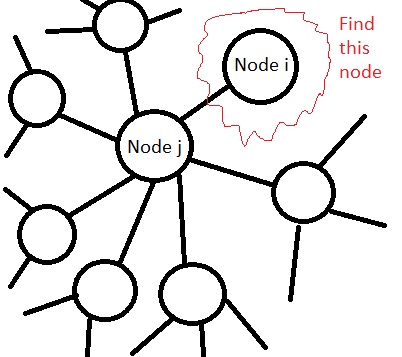
\includegraphics[scale=.5]{nodes.jpg}}
\caption{Objective is to find node $i$ having highest ${n_{s}}_i$}
\label{fig}
\end{figure}

Neighbor nodes having lower connection may influence these core nodes, less costly, and can have similar infection affect like high $k_{s}$ ones. Therefore, I assume to find a relation between $k$ and $k_{s}$ to inspect the influencer low k-valued neighbors. After my study, I derived a new attribute for nodes in $G_{gen}$. This attribute is called n-shell ($n_{s}$) and it mentions the strength of motivation to spend extra cost for this node, illustrated in Figure 1, to achieve a similar output from a core node. 


% ~~~~~~~~~~~~~~~~~~~~~~~~~~~~~~~~~~~~~~~ 
\section{Method for Study} 

At this study, I used Python 3 for coding network analyzing and programming tools. I intensely used NetworkX library $^{[2]}$ for graph analysis. I coded several python files to run algorithms for generating graph, k-shell decomposition, n-shell decomposition, SIR spread, and plotting for results. Relevant  python files are in attachment section of the report.

\subsection{Generating Graph}

As mentioned in the introduction section, due to computational constraints, I had to generate my own network ($G_{gen}$) instead of using networks mentioned at Kitsak's study. I used Python's NetworkX library $^{[2]}$, and applied an extended Barabási–Albert model graph. This is a built-in functionality of NetworkX. With this function, I generated random graphs, which are constructed using preferential attachment. This model allows new edges, rewired edges or new nodes. It constructs graph based on the probabilities $p$ and $q$ with $p+q<1$. The growing behavior of the graph is as follows:

\begin{itemize}
  \item With $p$ probability, new edges are added to the graph, starting from randomly chosen existing nodes and attached preferentially at the other end. 
  \item With $q$ probability, existing edges are rewired by randomly choosing an edge and rewiring one end to a preferentially chosen node.
  \item With $1-p-q$ probability, new nodes are added to the graph with edges attached preferentially.
\end{itemize}

By applying this algorithm into my generator code, I constructed 10 different graphs by using different values for $p$, $q$ and number of edges to connect randomly at time. The python file to generate the graphs is given in Attachment 1. 

I evaluated these graphs based on intensity of connections and number of shells to the core of the graph.  Table 1 shows summary of information about graphs generated.  From this list of graph, number of cores ($k_{s}$) and average degree ($k_{M}$) is the highest for ${G_{gen}}_6$. Therefore, I selected to run my analysis on \textbf{${G_{gen}}_6$} for the further part of the study. 


\begin{table} [h]
\begin{tabular}{|c|c|c|c|r|}
\hline
Graph & $N$ & $E$ & $k_{s}$ & $k_{M}$ \\
\hline
${G_{gen}}_1$ & 1,000 & 9,921 & 20& 19.84 \\
${G_{gen}}_2$  & 10,000 & 33,902 & 11 & 6.78 \\
${G_{gen}}_3$  & 20,000 & 109,386 & 14 &10.93 \\
${G_{gen}}_4$  & 100 & 558 & 12 &11.16 \\
${G_{gen}}_5$  & 1,000 & 7,570 & 19 &15.14 \\
${G_{gen}}_6$  & 1,000 & 38,168 & 105 &76.33 \\
${G_{gen}}_7$  & 500 & 6,080 & 32 &24.32 \\
${G_{gen}}_8$  & 1,000 & 8,070 & 20 &16.14 \\
${G_{gen}}_9$  & 1,000 & 16,224 & 47 &32.44 \\
${G_{gen}}_{10}$  & 2,000 & 16,835 & 26 &16.83 \\

\hline
\end{tabular}
\caption{Graphs generated with various combinations of $N$, $p$ and $q$}
\end{table}

\subsection{K-shell Decomposition}

In order to calculate $k_{s}$ values of the nodes in ${G_{gen}}_6$, I wrote a code in Python by applying the algorithm for k-shell composition detailed in Algorithm 1 $^{[3]}$. This code file is provided as Attachment 2. 

\begin{algorithm}
\SetAlgoLined
\KwResult{K-shell ($k_{s}$) for $G (V,E)$ undirected network }
 $C\gets V$\;
 $s\gets 0$\;
 $V_{s} = \emptyset$ \;
 \While{ $C  \neq \emptyset$ }{
   \While{ There are vertices of degree $s$ in $C$  }{	
	Select $i$ with degree $s$ in $C$\;
	 $C\gets C - \{ $i$ \} $\;
	 $V_{s} = V_{s} \cup \{ $i$ \} $\;
	Remove all edges of $i$\;
	Update the degrees in $C$\;
 }
 $s\gets s + 1$\;
 $V_{s} = \emptyset$ \;
}
$s:V \mapsto \mathbb{N}$ \;
$i \mapsto {k_{s}}_i$\;
 \caption{Algorithm for defining k-shell ($k_{s}$) value of a node}
\end{algorithm}

After decomposing shells of the graph, nodes are divided into 105 different shells. Table 2 demonstrates the number nodes in different shells. Since I used my own generated graph for analysis, I couldn't compare results for Kitsak's results. This is why I run my own results for $k_{s}$ against $c_{b}$ and $k$ in order to measure performance after spreading algorithm.

\begin{table} [h]
\centering
\begin{tabular}{|c|r|}
\hline
 $k_{s}$ Range & Number of $N$ \\
\hline
01-10&186\\
10-20&161\\
20-30&110\\
30-80&334\\
80-100&65\\
101&	1\\
102&	4\\
103&	1\\
104&	1\\
105&	137\\
\hline
\end{tabular}
\caption{Number of nodes in different $k_{s}$ ranges}
\end{table}



\subsection{Spreading Algorithm for Susceptible – Infectious – Recovered (SIR) }

I applied the susceptible – infectious – recovered (SIR) algorithm to study the spreading process. This model can be describe as disease spreading, or information and rumor spreading in social processes. In this algorithm, we define a probability ($p$) that an infectious node will infect a susceptible neighbor. The value of the probability is important during the analysis. If you apply large values, there is a risk of spreading to large portion of population, so you cannot observe a significant difference regarding origin of the spread. Therefore, I simulated by study with small values as $p$:\{ 0.005, 0.01, 0.015, 0.025, 0.05 \}.

Since this model is  stochastic model, I applied the algorithm for each case in 100 runs. I construct a python code for this iterative run. The python file for the algorithm is provide in Attachment 3. 

The model I studied assumes that infected nodes are recovered after the cycle that it interacts within the neighbors once, and spread is triggered from a single node ($i$). I didn't apply a probabilistic approach on recovery, so if a node $i$ is infected, then it will be recovered eventually. Algorithm 2 illustrates the flow of the process.

\begin{algorithm}
\SetAlgoLined
\KwResult{SIR for $G (V,E)$ undirected network  }
Let $i \in V$\;
$I$: Set of current spreaders\;
$R$: Set of recovered\;
$N(i)$: Set of neighbors of $i$\;
$\beta$: Probability of spreading infection\;
$I = \{ i \}$,   $R = \emptyset$ \;
 \While{ $I  \neq \emptyset$ }{
	Select $j \in V$\;
	$I\gets I - \{ $j$ \} $\;
	$R = R \cup \{ $j$ \} $\;
	$C = N(j)   \smallsetminus (I  \cup R ) $\;
   \While{ $C  \neq \emptyset$ }{	
	Select $l \in C$\;
	 $C\gets C - \{ $l$ \} $\;
	Infect $l$ with probability of $\beta$\;
	  \If{ $l$ is infected}{
		$I \gets I \cup \{ $l$ \} $\;
	   }
     }
}
Spread Ratio ($r$) is ratio of recovered nodes $R$ againts all nodes in $V$ \;
 \caption{Spreading algorithm of Susceptible – Infectious – Recovered (SIR)}
\end{algorithm}

After I run the code for 100 iterations, I could simulated similar outputs that Kitsak presented his study [1] with my generated graph . Considering 5 different probabilities ($p$:\{ 0.005, 0.01, 0.015, 0.025, 0.05 \}), I received the similar result. There are significant improvement on infection rate when  $k_{s}$ increased, while it doesn't have significance impact on performance when you increase the $c_{b}$ or $k$ values in same $k_{s}$. Figure 2 has a sample illustration of results achieved. Figures for other $p$ values are provided in Attachment 4. 

\begin{figure}[h]
\begin{subfigure}{.5\textwidth}
	\centerline{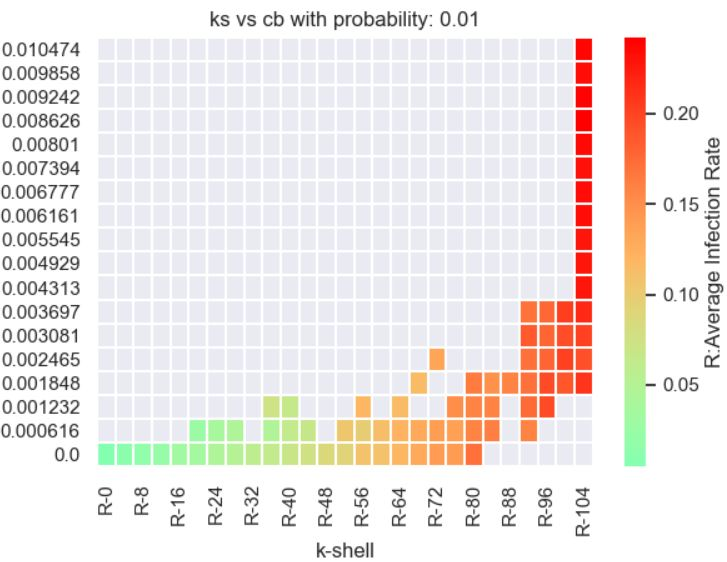
\includegraphics[scale=.5]{ks-cb-01.jpg}}
	\caption{$c_{b}$ against $k_{s}$ at $p=0.01$}
	\label{fig:fig1}
\end{subfigure}
\begin{subfigure}{.5\textwidth}
	\centerline{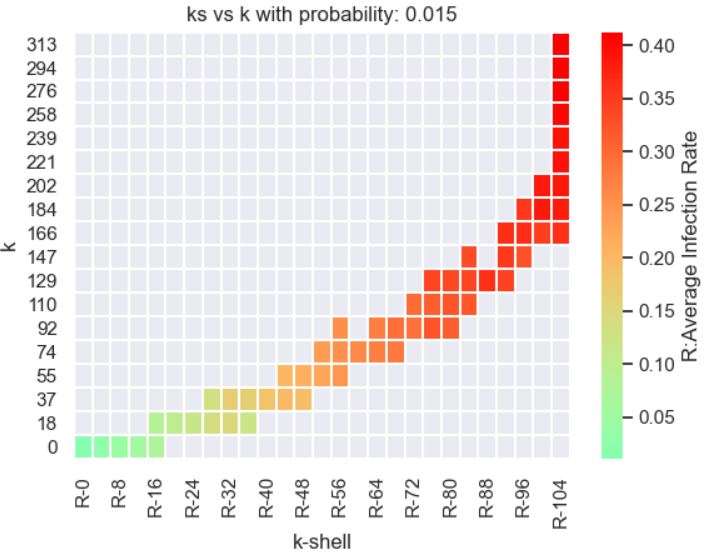
\includegraphics[scale=.5]{ks-k-015.jpg}}
	\caption{$k$ against $k_{s}$ at $p=0.015$}
	\label{fig:fig2}
\end{subfigure}
\caption{Comparison of spreading performances}
\label{fig:fig}
\end{figure}



\subsection{Algorithm for n-shell decomposition}

Since the graph I studied provided similar results with Kitsak paper, then I focus on the question of finding efficient spreader interrelated with neighbors having highest $k_{s}$ values. I used a attribute \textbf{\textit{neighborhood-to-shell}} (n-shell) to differentiate nodes from each other. I represent this value as ${n_{s}}_i$, n-shell value of node $i$.

To compute the n-shell, there are three critical parameters: k-shell, degree of node, and number of nodes that has a common relationship. I initially set all $n_{s}$ equal to $k_{s}$, so all the nodes should have at least a value equal to its k-shell value. 

As illustrated at Figure 1, main objective is to find nodes which are located to strategically closer to core nodes. As explained by Kitsak, highest $k_{s}$ values have better impact on spreading than highest degree ones. Therefore, neighbors of these highest $k_{s}$ nodes are potential. Since I focus on cost effective spreaders, from these neighbors I spotlighted the ones having lowest $k$ values. Here, there is another factor: how many nodes sharing the same highest $k_{s}$ valued node. I formulated the relationship of these parameters as follows for node $i$ which is the neighbor of node $j$:

\[
{n_{s}}_i = \ln{(\frac{k_{j}}{k_{i}})}{k_{s}}_j
\]

\begin{algorithm}
\SetAlgoLined
\KwResult{$n_{s}$ for $G (V,E)$}
Let $i \in V$\;
$N(i)$: Set of neighbors of $i$\;
${n_{s}}_i\gets {k_{s}}_i : \forall i \in V $\;
$C = V$ \;
 \While{ $C  \neq \emptyset$ }{
	Select $i \in C$\;
	$C\gets C - \{ $i$ \} $\;
	$A = N(j) $\;
   \While{ $A  \neq \emptyset$ }{	
	Select $j \in A$\;
	 $A\gets A - \{ $j$ \} $\;
	Calculate formula ${n_{s}}_j = \ln{(\frac{k_{i}}{k_{j}})}{k_{s}}_i$\;
	  \If{ Calculation is greater than ${n_{s}}_i$}{
		${n_{s}}_j \gets Calculated Value$\;
	   }
     }
}
 \caption{Algorithm for assigning $n_{s}$ for each node $i$}
\end{algorithm}

In order to compute this ratio and assign to each node, I coded python file using Algorithm 3. 
With this formula, being a neighbor to a node having high $k_{s}$, having a low degree ( meaning your connection to this neighbor is import for that node), and interacting to a neighbor with having large connection becomes significant. In order to increase prioritization of k-shell and balance the affect of other two parameters, I utilized logarithmic effect on the ratio.

After running this code on the SIR results,  I draw graphs showing relationship between  $k_{s}$ and $n_{s}$. Figure 3 illustrates this relationship for two different probabilities. 

\begin{figure}[h]
\begin{subfigure}{.5\textwidth}
	\centerline{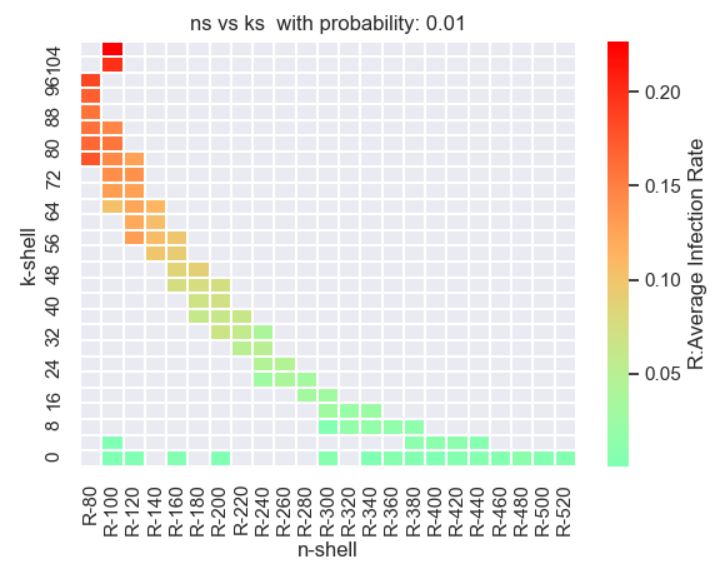
\includegraphics[scale=.5]{ns-ks-01.jpg}}
	\caption{$n_{s}$ against $k_{s}$ at $p=0.01$}
	\label{fig:fig1}
\end{subfigure}
\begin{subfigure}{.5\textwidth}
	\centerline{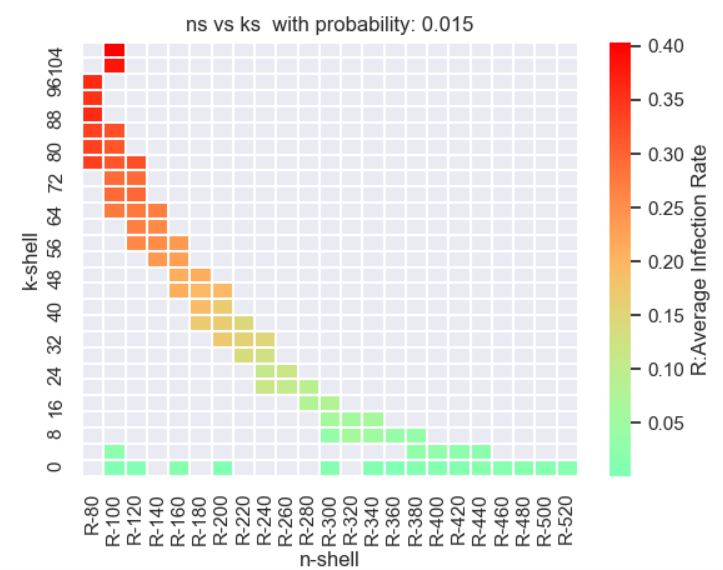
\includegraphics[scale=.5]{ns-ks-015.jpg}}
	\caption{$n_{s}$ against $k_{s}$ at $p=0.015$}
	\label{fig:fig2}
\end{subfigure}
\caption{Comparison of $k_{s}$ and $n_{s}$}
\label{fig:fig}
\end{figure}

As seen in the figures, for the nodes having  $n_{s}$ values greater than $300$ has low values on both $k_{s}$. This means that they are connected to some higher $k_{s}$ nodes. However, as seen at average infection rate, they don't have significant affect on spreading. At the next section, I will focus on question whether the spread rate is affected if there is a motivation factor for these high $n_{s}$ node by assigning them different probability.

% ~~~~~~~~~~~~~~~~~~~~~~~~~~~~~~~~~~~~~~~ 
\section{Motivation Factor for high $n_{s}$ nodes} 

As discussed at the beginning of this paper, in equal spreading conditions (same $p = \beta$), higher $k_{s}$ valued nodes have better performance on spreading if they are originator of the spread. However, it's also known that reaching a node with higher $k_{s}$ also cost higher than other nodes. This case can be validated with real-life problems such as advertising a new product.

 Therefore, I analyze whether will there be any significant change on spreading ratio, if I apply a "higher" probability of spread ratio for only the originator node, and same probability for the rest, if the spread is originated from a node having $n_{s}$ values greater than $300$.

In order to apply this approach, I have modified the SIR algorithm. With this change, algorithm gets two probability parameters: ${\beta}_{1}$ and ${\beta}_{2}$. ${\beta}_{1}$ represents probability of infection for only spread's starting node, whereas ${\beta}_{2}$ is the rate of infection for all other nodes. Algorithm 4 illustrates the updated SIR algorithm.

\begin{algorithm}
\SetAlgoLined
\KwResult{SIR for $G (V,E)$ undirected network  }
Let $i \in V$\;
$I$: Set of current spreaders\;
$R$: Set of recovered\;
$N(i)$: Set of neighbors of $i$\;
$\beta$: Probability of spreading infection\;
${\beta}_{1}$: Probability of spreading infection from origin\;
${\beta}_{2}$: Probability of spreading infection for rest\;
$I = \{ i \}$,   $R = \emptyset$ \;
 \While{ $I  \neq \emptyset$ }{
	Select $j \in V$\;
	  \eIf{ $j$ is i}{
		$\beta \gets {\beta}_{1} $\;
	   }{
		$\beta \gets {\beta}_{2} $\;
	   }
	$I\gets I - \{ $j$ \} $\;
	$R = R \cup \{ $j$ \} $\;
	$C = N(j)   \smallsetminus (I  \cup R ) $\;
   \While{ $C  \neq \emptyset$ }{	
	Select $l \in C$\;
	 $C\gets C - \{ $l$ \} $\;
	Infect $l$ with probability of $\beta$\;
	  \If{ $l$ is infected}{
		$I \gets I \cup \{ $l$ \} $\;
	   }
     }
}
Spread Ratio ($r$) is ratio of recovered nodes $R$ againts all nodes in $V$ \;
 \caption{Alternative Spreading algorithm of SIR with different spread probability of seed node}
\end{algorithm}

After modifying the code for simulation, I recalculated infection rates for spread originated from high $n_{s}$ valued nodes. I make the iterations with the parameters belows:

\begin{itemize}
  \item ${\beta}_{1} = 0.25$ and ${\beta}_{2} = 0.01$ 
  \item ${\beta}_{1} = 0.5$ and ${\beta}_{2} = 0.01 $ 
  \item ${\beta}_{1} = 0.25$ and ${\beta}_{2} = 0.005$ 
  \item ${\beta}_{1} = 0.5$ and ${\beta}_{2} = 0.005 $ 
\end{itemize}

I choose small ${\beta}_{2}$ values intentionally to observe whether there will be significant change on infection even though spread origins have low $k_{s}$ values. 

After running the simulation with updated SIR algorithm, results shown in Figure 4 and 5 are achieved. 

In Figure 4, there is a comparison between original k-shell comparison simulation with  ${\beta}_{2} = 0.01$ and modified SIR simulation with a motivation factors for the nodes having  $n_{s}$ values greater than $300$. In the second cases, spread probability from these nodes are increased significantly with a cost of $C_m$. As seen in the figure 4, after increasing the probability of spread for origin only, higher $n_{s}$ nodes has reached the infection rates of these nodes are significantly increased and reached to level similar to high $k_{s}$ nodes. If the motivation factor is increased to higher level, the expectation to have higher infection rate with higher $n_{s}$ increases.

\begin{figure}[h]
\begin{subfigure}{.5\textwidth}
	\centerline{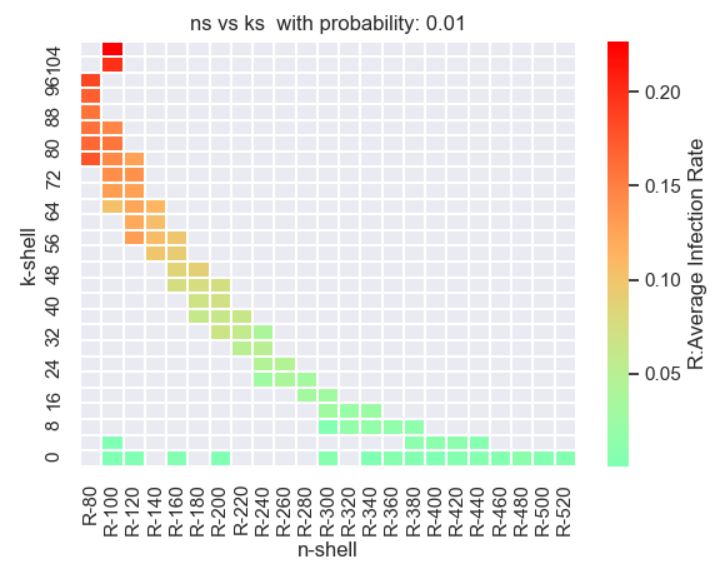
\includegraphics[scale=.4]{ns-ks-01.jpg}}
	\caption{$n_{s}$ against $k_{s}$ at $p=0.01$}
	\label{fig:fig1}
\end{subfigure}
\begin{subfigure}{.5\textwidth}
	\centerline{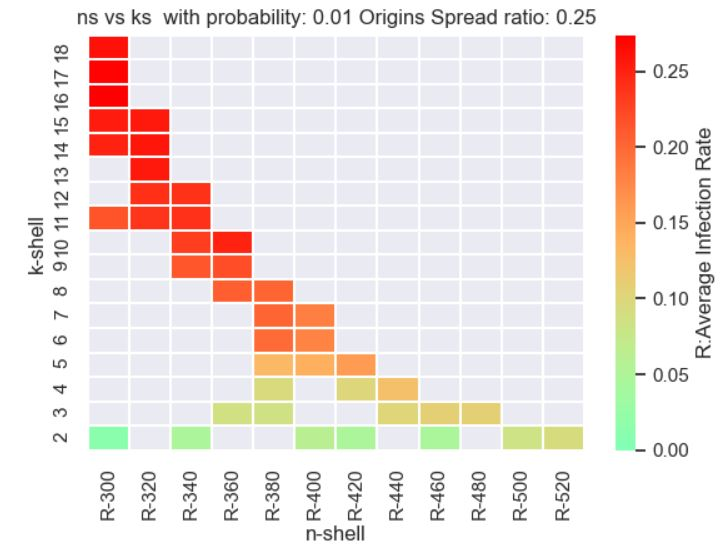
\includegraphics[scale=.4]{ns-ks-01-25.jpg}}
	\caption{$n_{s}$ against $k_{s}$ at ${\beta}_{1} = 0.25$ }
	\label{fig:fig2}
\end{subfigure}
\begin{subfigure}{.5\textwidth}
	\centerline{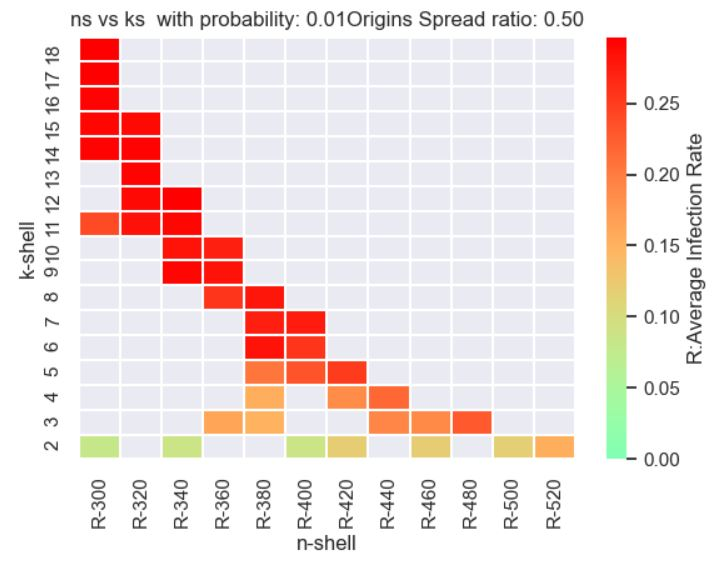
\includegraphics[scale=.4]{ns-ks-01-50.jpg}}
	\caption{$n_{s}$ against $k_{s}$ at ${\beta}_{1} = 0.50$}
	\label{fig:fig2}
\end{subfigure}
\caption{Comparison of $k_{s}$ and $n_{s}$}
\label{fig:fig}
\end{figure}

As seen in Figure 5, even at a small rate of infection such as $p=0.005$, if you apply a motivation factor for origin of spreads having small  $k_{s}$ or  $k$ values, it's possible to exceed performance of high  $k_{s}$ valued nodes.  

\begin{figure}[h]
\begin{subfigure}{.5\textwidth}
	\centerline{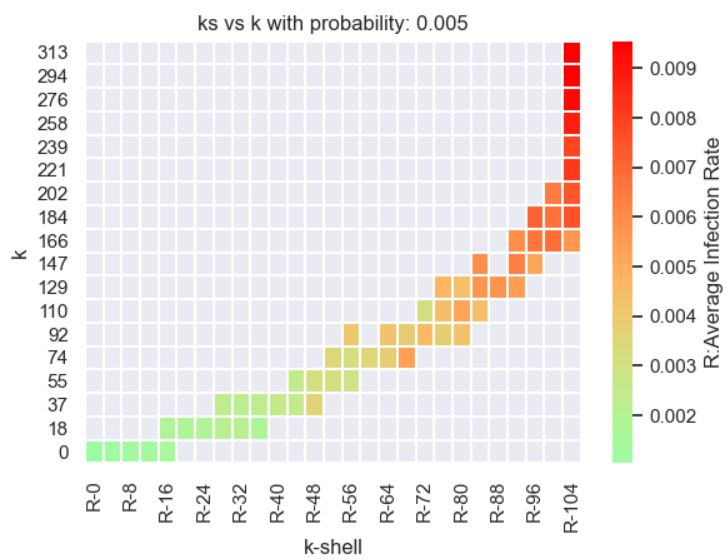
\includegraphics[scale=.4]{ks-k-005.jpg}}
	\caption{$k$ against $k_{s}$ at $p=0.005$}
	\label{fig:fig1}
\end{subfigure}
\begin{subfigure}{.5\textwidth}
	\centerline{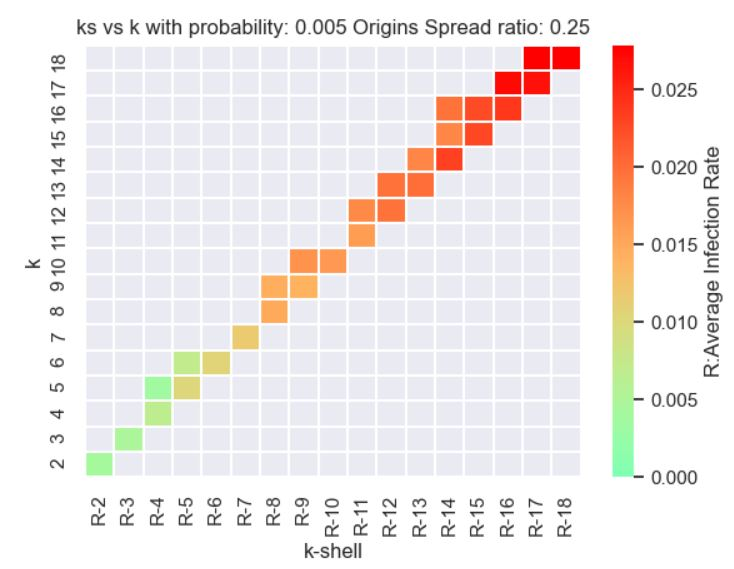
\includegraphics[scale=.4]{ks-k-005-25.jpg}}
	\caption{$k$ against $k_{s}$ at ${\beta}_{1} = 0.25$}
	\label{fig:fig2}
\end{subfigure}
\begin{subfigure}{.5\textwidth}
	\centerline{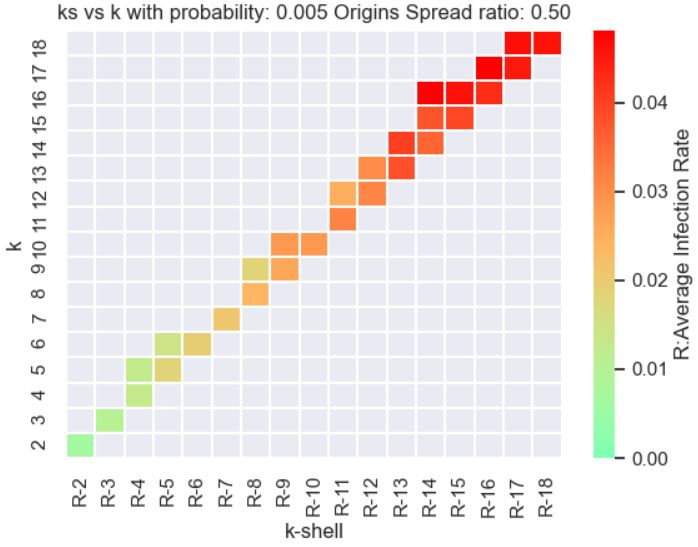
\includegraphics[scale=.4]{ks-k-005-50.jpg}}
	\caption{$k$ against $k_{s}$ at ${\beta}_{1} = 0.50$}
	\label{fig:fig2}
\end{subfigure}
\caption{Comparison of $k$ and $k_{s}$}
\label{fig:fig}
\end{figure}

Other figures related to this comparison for  $k$ , $k_{s}$ and  $k$ and $k_{s}$ is also provided at Attachment 4.  Moreover, simulation results for each node and case is also provided in Attachment 5.

\section{Conclusion} 

In this project paper, I analyzed a network to find an alternative approach for finding a less costly and more effective influencer. To achieve this  I utilized the k-shell approach, degree of node and number of neighbor connections together, and I construct a formula to calculate a new attribute, $n-shell$. 
\[
{n_{s}}_i = \ln{(\frac{k_{j}}{k_{i}})}{k_{s}}_j
\]
Moreover, by modifying the SIR algorithm, I applied a new parameter origin infection probability, into my simulations. This helped me to analyze whether there are any positive correlation if a motivation factor is applied for infection probability of origin spreader. In my study, I observed that it's possible to reach similar or better spreading performances than high $k_{s}$ nodes, if you increase spreading probability of high $n_{s}$ nodes. However, motivation cost $C_{m}$ should not exceed to cost of spreading from higher $k_{s}$ nodes, $C_{k_{s}}$. To sum up, n-shell approach can be further studied considering cost relationship as well.

\section{References} 

{\footnotesize [1] Maksim Kitsak, Lazaros K. Gallos, Shlomo Havlin, Fredrik Liljeros, Lev Muchnik,H. Eugene Stanley and Hernán A. Makse, \textit{Identification of influential spreaders in complex networks}, Nature Physics, 2010 }
{\footnotesize [2] Network X: Network Analysis in Python \textit{https://networkx.org/}
{\footnotesize [3] SWE580 Complex Network Course notes \textit{https://www.cmpe.boun.edu.tr/courses/cmpe556/}

\section{Attachments} 

{\footnotesize [1] Python code to generate graphs with extended Barabási–Albert model}
{\footnotesize [2] Python code for k-shell decomposition}
{\footnotesize [3] Python code for spreading algorithm of Susceptible – Infectious – Recovered (SIR) }
{\footnotesize [4] Figures for infection rates at different probability combinations}
{\footnotesize [5] Simulation Results}

% ~~~~~~~~~~~~~~~~~~~~~~~~~~~~~~~~~~~~~~




%% ~~~~~~~~~~~~~~~~~~~~~~~~~~~~~~~~~~~~~~~ 
%\bibliographystyle{ieeetr}
%
%\bibliography{bingol-template-project-report}




% ~~~~~~~~~~~~~~~~~~~~~~~~~~~~~~~~~~~~~~~ 
\end{document}